 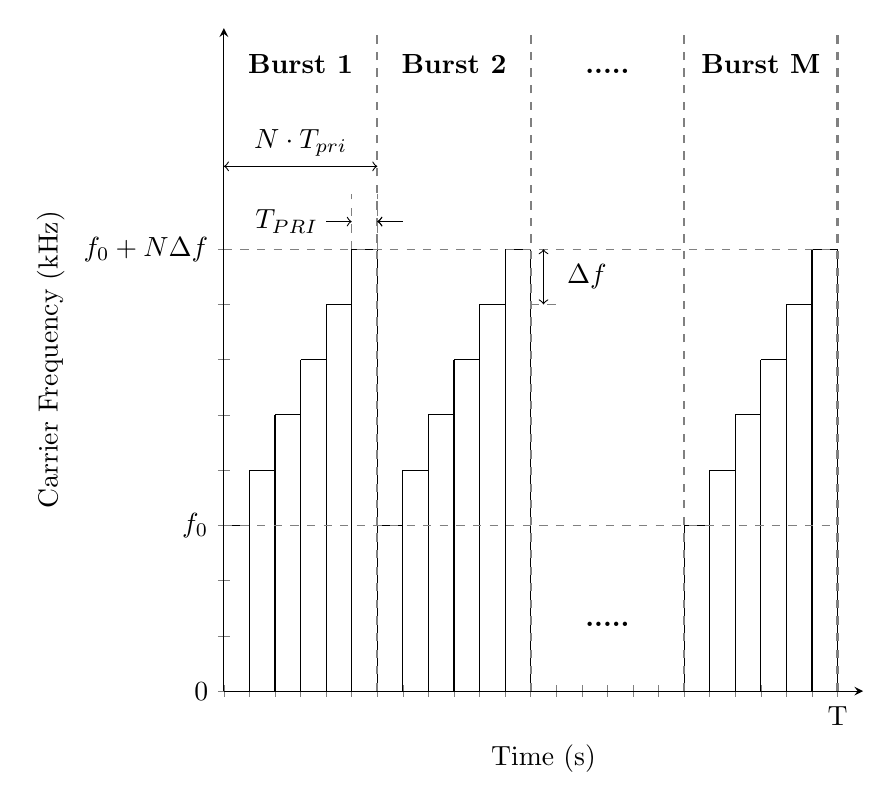
\begin{tikzpicture}    
        \begin{axis}[
            width=0.8\textwidth,
            height=10cm,
            xlabel={Time (s)},
            ylabel={Carrier Frequency (kHz)},
            axis lines=left,
            %grid=both,
            xmin=0,
            xmax=1.25,
            ymin=0, % Start from y=0
            ymax=12,
            xtick={0, 0.05, 0.1, 0.15, 0.2, 0.25, 0.3,0.35,0.4,0.45,0.5,0.55,0.6,0.65,0.7,0.75,0.8,0.85,0.9,0.95,1,1.05,1.1,1.15,1.2},
            xticklabels={,,,,,,,,,,,,,,,,,,,,,,,,T}, % Remove x-axis tick labels
            ytick={0, 1, 2, 3, 4, 5, 6,7,8},
            yticklabels={0, , , $f_0$, , , , , $f_0 + N\Delta f$}, % Modify y-axis tick labels
        ]
        
        % Step graph
        \addplot[black, jump mark left] coordinates {
            (0, 3)
            (0.05, 4)
            (0.1, 5)
            (0.15, 6)
            (0.2, 7)
            (0.25, 8)% End point of burst 1
            (0.3, 3)
            (0.35, 4)
            (0.4, 5)
            (0.45, 6)
            (0.5, 7)
            (0.55, 8)
            (0.6,8)% End point of burst 2
            
            (0.9, 3)
            (0.95, 4)
            (1, 5)
            (1.05, 6)
            (1.1, 7)
            (1.15, 8)
            (1.2,8)% End point of burst N
        };
        \addplot[black, ycomb] coordinates {
            (0, 3)
            (0.05, 4)
            (0.1, 5)
            (0.15, 6)
            (0.2, 7)
            (0.25, 8)% End point of burst 1
            (0.3, 8)
            (0.35, 4)
            (0.4, 5)
            (0.45, 6)
            (0.5, 7)
            (0.55, 8)
            (0.6,8)% End point of burst 2
            
            (0.9, 3)
            (0.95, 4)
            (1, 5)
            (1.05, 6)
            (1.1, 7)
            (1.15, 8)
            (1.2,8)% End point of burst N
        };
        \addplot[gray,ycomb, mark=none, thick, dashed] coordinates{
            (0.3,12)
            (0.6,12)
            (0.9,12)
            (1.2,12)
        };
       
        % Label max and f0 frequency
        \draw[gray, dashed, -] (axis cs: 0, 3) -- (axis cs: 1.2, 3);
        \draw[gray, dashed, -] (axis cs: 0, 8) -- (axis cs: 1.2, 8);

        % Label frequency step
        \draw[gray, dashed, -] (axis cs: 0.6, 7) -- (axis cs: 0.65, 7);
        \draw[<->] (axis cs: 0.625, 7) -- (axis cs: 0.625,8) node[midway,right, xshift=5pt] {\textbf{$\Delta f$}} ;
         
        % Label period
        \draw[gray, dashed, -] (axis cs: 0.25, 8) -- (axis cs: 0.25, 9);
        \draw[gray, dashed, -] (axis cs: 0.3, 8) -- (axis cs: 0.3, 9);
        \draw[->] (axis cs: 0.2, 8.5) -- (axis cs: 0.25, 8.5) node[midway,left,xshift=-4pt] {$T_{PRI}$};
        \draw[<-] (axis cs: 0.3, 8.5) -- (axis cs: 0.35, 8.5) ;

        % Label PRI
        \draw[<->] (axis cs: 0, 9.5) -- (axis cs: 0.3, 9.5) node[midway,above] {$N \cdot T_{\gls{pri}}$};
        \draw[<-] (axis cs: 0.3, 8.5) -- (axis cs: 0.35, 8.5) ;

        %Label Bursts
        \draw[draw=none] (axis cs: 0, 11) -- (axis cs: 0.3, 11) node[midway,above] {\textbf{Burst 1}};
        \draw[draw=none] (axis cs: 0.3, 11) -- (axis cs: 0.6, 11) node[midway,above] {\textbf{Burst 2}};
        \draw[draw=none] (axis cs: 0.9, 11) -- (axis cs: 1.2, 11) node[midway,above] {\textbf{Burst M}};

        % Label ...
        \draw[draw=none] (axis cs: 0.6, 11) -- (axis cs: 0.9, 11) node[midway,above] {\textbf{.....}};
        \draw[draw=none] (axis cs: 0.6, 1) -- (axis cs: 0.9, 1) node[midway,above] {\textbf{.....}};
        \end{axis}
        
    \end{tikzpicture}